
\begin{partbacktext}
\part{Recovery Modeling}

This section provides an introductory discussion on the modeling of disaster recovery for infrastructure, residential buildings, businesses, and communities. The aim of this section is not to present an exhaustive list or propose an ideal approach given the complexity of the recovery process and the wide variation across hazard types and geographies. Empirical studies are reviewed to identify factors that are associated with recovery, providing the basis for conceptual models of recovery. It is also noted that, although, recovery simulations are often used to obtain proxies of the disaster resilience, disaster recovery is only one among many metrics of resilience \citep{national2019building,kwasinski2016conceptual}. For this reason, the scope of this section does not include a comprehensive review of the broader topic of disaster resilience.\

Disaster recovery modeling consists of assessing over time the performance of a system subjected to a shock. Prior to the shock, the system has a baseline state, $Q_b$. At the time of the event, $t_0$, disturbances to the system reduce its functionality to a new state, $Q_0$. Subsequently, the system is restored until a time $t_R$ when its new normal is established. Recovery may be partial, with the new normal below the pre-disaster state. Or, improvements may be done to the system and the new normal is an improvement. While comparing recovery with pre-disaster state is a common practice, another alternative is to compare it to the projected state of the system had the shock not occurred. Plotting the state of the system over time, $Q(t)$, against the time since the shock provides a graph as the one shown in Figure \ref{fig:ResilienceTriangle}. The curve $Q(t)$ is called the recovery trajectory \citep{Bruneau2003}. While loss assessments focus on the magnitude of the initial drop in the functionality of the system, recovery modeling is devoted to simulating the recovery trajectory. Hence, the main output from a recovery model is the time series of $Q(t)$.\

\begin{figure}[htb]
    \centering
    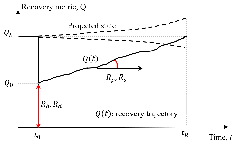
\includegraphics[width=0.7\textwidth, angle = 0]{Recovery/Resilience_Concepts.pdf}
    \caption{Resilience triangle. Adapted from \cite{Bruneau2003}.}
    \label{fig:ResilienceTriangle}
\end{figure}

The magnitude of the initial drop at $t_0$ is a function of the robustness, $R_b$, and the redundancy, $R_d$, of the system. A perfectly robust system is one that can experience a shock without significant changes. A perfectly redundant system is one that, if disrupted, can immediately and cost effectively rearrange itself to provide the same level of service as before the event. The ability of the system to regain functionality can be estimated from the slope of the recovery trajectory. The slope is influenced by the capacity of the system to mobilize resources and meet priorities. These are often called the system's resourcefulness, $R_s$, and rapidity, $R_p$ \citep{Bruneau2003}. The concepts in Figure \ref{fig:ResilienceTriangle} can be employed to study the recovery of critical infrastructure, housing, and businesses. The following sections discuss the state of the art in simulation the recovery of these three systems.\

\FloatBarrier
\end{partbacktext}
